\subsection{DOP 27 Комбинаторные методы нахождения оптимального пути в графе.}

\textbf{Определения}

\begin{itemize}
    \item Взвешенный орграф $G = (V, E, c)$ называется \textit{сетью} ($c$ --- функция, определяющая вес ребра).
    \item Ориентированный маршрут называется \textit{путем}. 
    \item Пусть $P$ --- некоторый $(v, w)$-путь: $v = v 0 \rightarrow v_1 \rightarrow \dots \rightarrow v_k = w$. Тогда $l(P) = c(e_1) + c(e_2) + \dots + c(e_k)$ называется длиной пути $P$, где $e_i$ --- ребро перехода от вершины $v_{i-1}$ к вершине $v_i$. 
    \item $(u, w)$-путь с наименьшей длиной называется \textit{кратчайшим}.
    \item Задача о кратчайшем пути между фиксированными вершинами: в заданной сети $G$ с двумя выделенными вершинами $s$ и $t$ найти кратчайший $(s, t)$-путь.
\end{itemize}

\textbf{Алгоритм Беллмана-Форда.} 
Сложность $\mathcal{O}(|V| + |E|)$.

Пусть мы хотим найти длину кратчайшего пути из $s$ в остальные вершины. Обозначим через $a_{kp}$ длину кратчайшего пути из $s$ в $p$, состоящего из $k$ дуг, или $\inf$, если такого пути не существует.

\textit{Инициализация}. 
$a_{0s} = 0$, $a_{0p} = \inf$ для всех вершин $p != k$.

\textit{Шаг алгоритма}.
Зная все минимальные длины путей из $k-1$ дуг, посчитать минимальную длину пути из $k$ дуг можно, перебрав все вершины, из которых имеются дуги, идущие в данную. Для всех вершин $p$: $a_{kp} = min\{a_{k-1,p'} + c((p',p))~|~p' \in V, (p',p) \in E\}$. 

Шаг повторяется $|V| - 1$ раз, так как если путь содержит больше дуг, то в нем точно имеется цикл, который можно выбросить. На практике нет необходимости хранить всю матрицу целиком, нужно хранить лишь три строки - ранее вычисленную $a_{k-1}$, вычисляемую сейчас $a_k$, и строку с ответами, которая обновляется на кажом шаге: $ans_p = min\{ans_p, a_{kp}\}$.

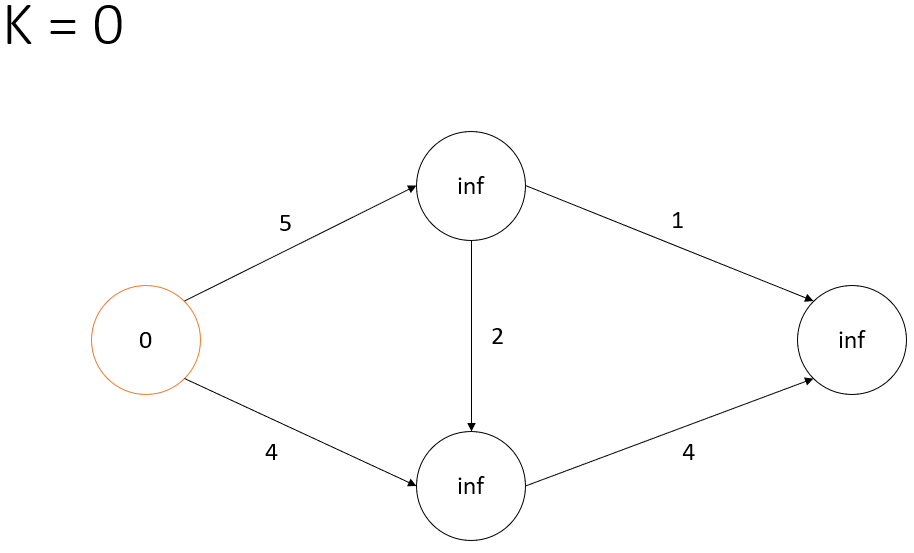
\includegraphics[width=0.9\columnwidth]{pics/dop28_1.png}

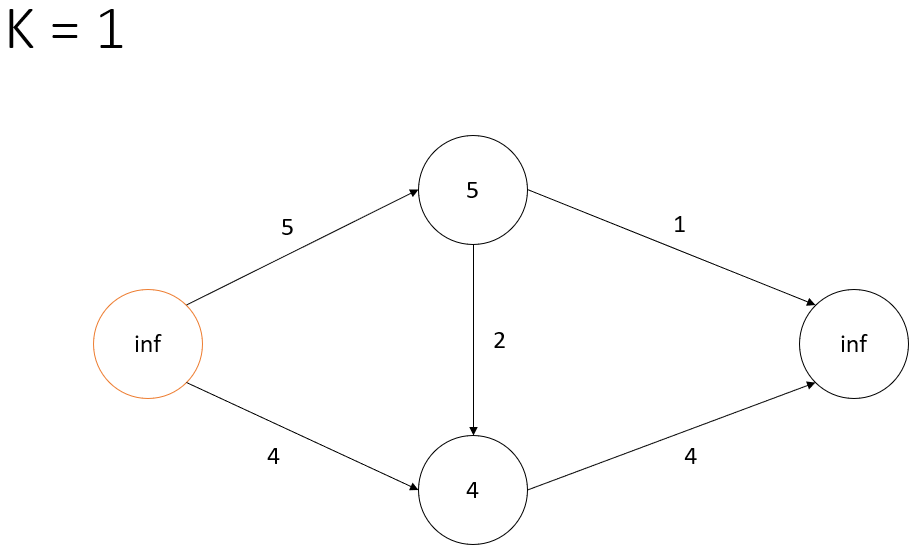
\includegraphics[width=0.9\columnwidth]{pics/dop28_2.png}

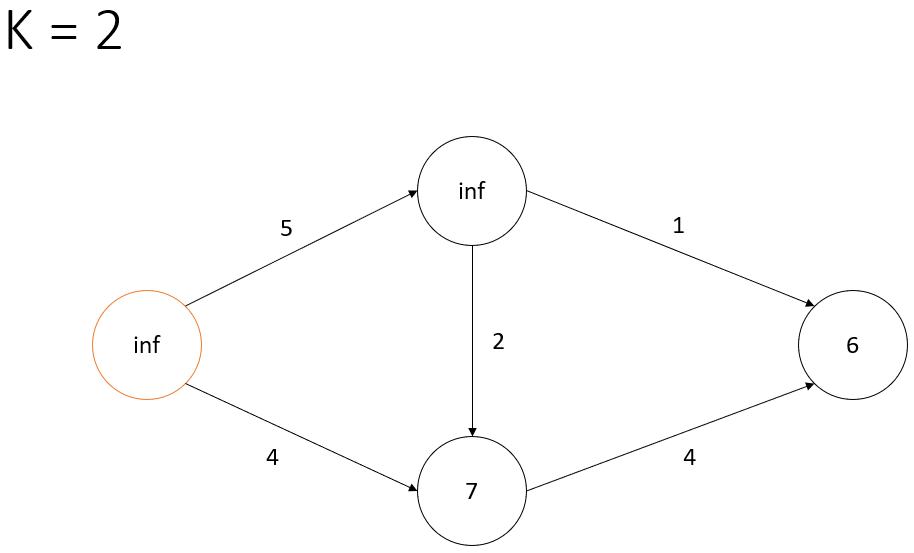
\includegraphics[width=0.9\columnwidth]{pics/dop28_3.png}

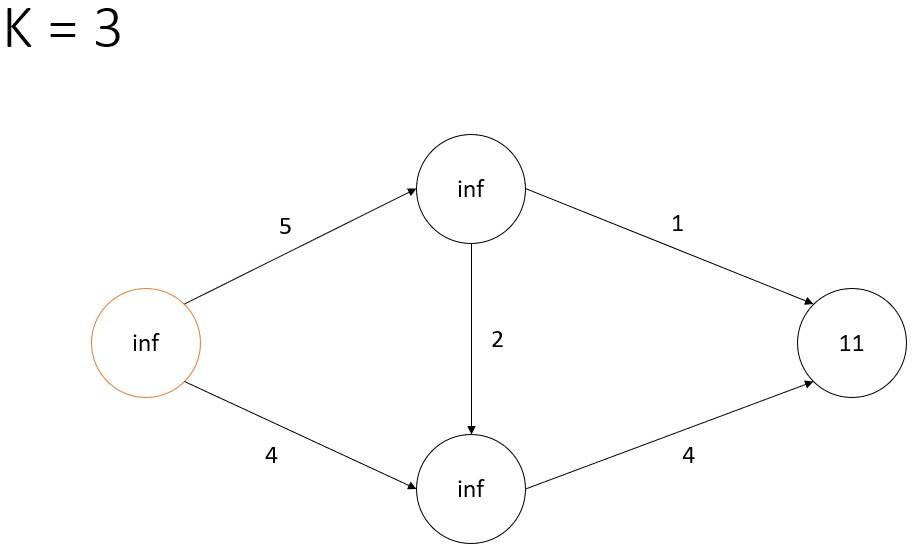
\includegraphics[width=0.9\columnwidth]{pics/dop28_4.png}

\textbf{Алгоритм Дейкстры.} 
Сложность варьируется (см. ниже). 

Каждой вершине из $V$ сопоставим метку --- минимальное известное расстояние от этой вершины до $s$. 
Алгоритм работает пошагово --- на каждом шаге он посещает одну вершину и пытается уменьшать метки. 
Работа алгоритма завершается, когда все вершины посещены.

\textit{Инициализация}. 
Метка самой вершины $s$ полагается равной 0, метки остальных вершин --- $\inf$.
Это отражает то, что расстояния от $s$ до других вершин пока неизвестны. 
Все вершины графа помечаются как непосещённые.

\textit{Шаг алгоритма}. 
Если все вершины посещены, алгоритм завершается. 
В противном случае, из ещё не посещённых вершин выбирается вершина $u$, имеющая минимальную метку. 
Обновим метки соседних с $u$ вершин - $\forall s: (u,s) \in E: label_s = min\{label_s, label_u + c((u, s))\}$
Пометим вершину $u$ посещенной.

Сложность алгоритма варьируется в зависимости от того как хранить множество непосещенных вершин для удобства получения вершины с минимальной веткой. При хранении множества как списка, упорядоченного по убыванию меток, сложность алгоритма состявляет $\mathcal{O}(|V|^2)$. При использовании двоичной кучи сложность уменьшается до $\mathcal{O}((|E| + |V|) \log|V|)$.

% \todo{у черепниной и фелорова есть картинки для дейкстры, но они не влезают}

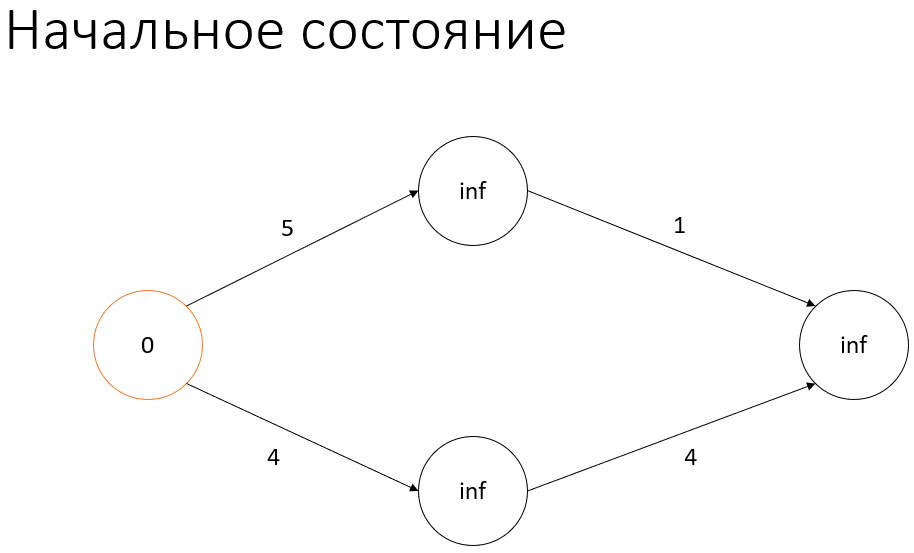
\includegraphics[width=0.6\columnwidth]{pics/29___0.png}

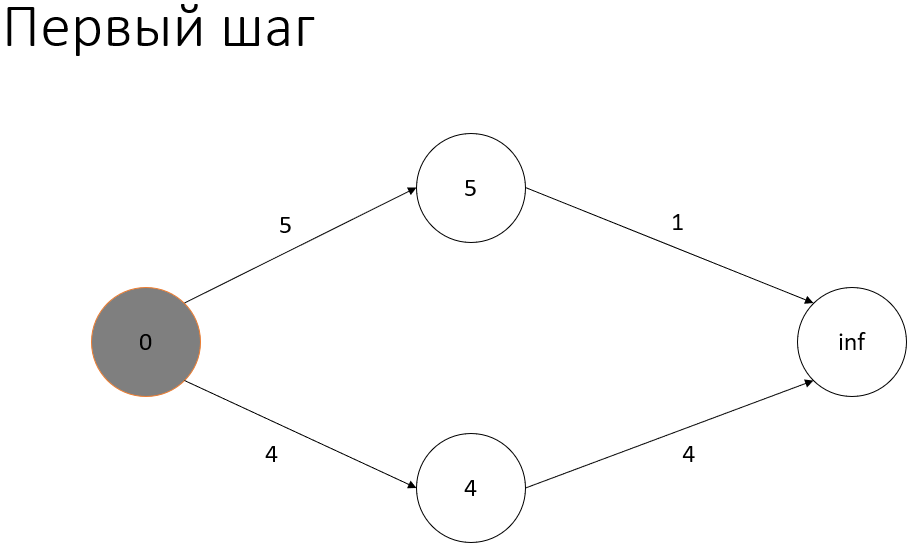
\includegraphics[width=0.6\columnwidth]{pics/29___1.png}

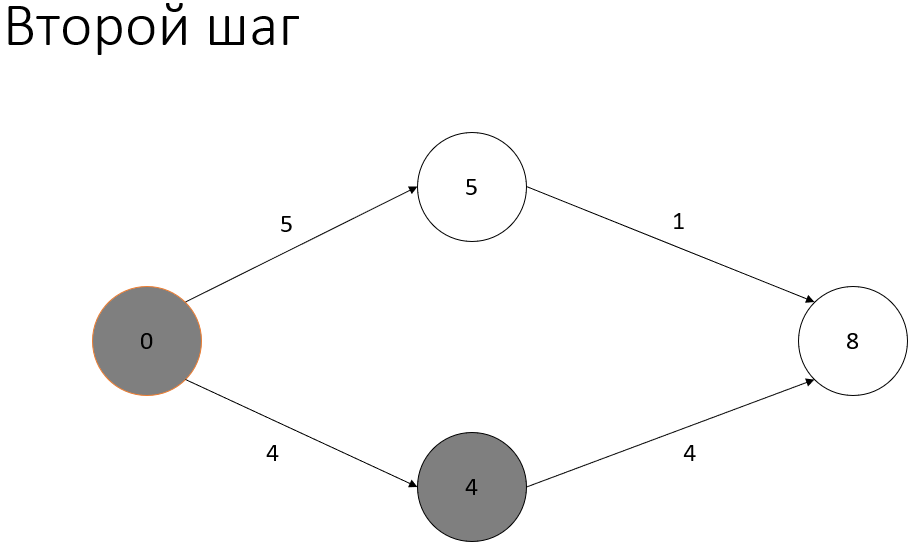
\includegraphics[width=0.6\columnwidth]{pics/29___2.png}

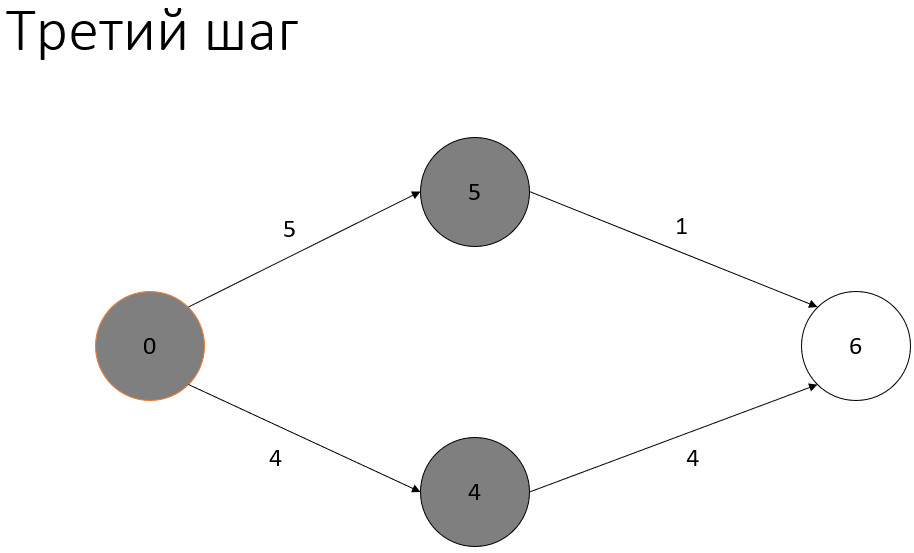
\includegraphics[width=0.6\columnwidth]{pics/29___3.png}

Четвертый шаг:

+ серенький последний круг

% -------- source --------
\bigbreak
[\cite[page 69-96]{replace_me}]
